\chapter{Reviewing Friedmann, Adding Radiation, and Finding Dark Matter}

This chapter follows Leonard Susskind's third lecture on cosmology, with the surviving board images retained where the blackboard itself carries part of the mathematical argument. The lecture begins in deliberate review mode. We rebuild the Friedmann equation from a homogeneous Newtonian picture, reinterpret its source as energy density rather than mere rest mass, compare matter-dominated and radiation-dominated expansion, and then turn outward to the surface of last scattering and to the astronomical evidence for dark matter. The underlying lecture is due to Leonard Susskind, and the transcript-and-frame curation owes an explicit debt to LazyingArt LLC and Video2Book.

\section{Homogeneity, Comoving Coordinates, and the Newtonian Setup}

On scales large compared with clusters of galaxies, the lecture treats the universe as approximately homogeneous. Once we make that approximation, we may choose ourselves to sit at the origin of coordinates without loss of generality. Susskind then places a representative galaxy, or if we prefer a purely imaginary test particle moving with the cosmic flow, at comoving coordinate \(x=1\).

This is the useful normalization. If the particle is at \(x=1\), then its physical distance from us is by definition the scale factor \(a(t)\). A particle at \(x=2\) is twice as far away, at distance \(2a(t)\), and so on. The scale factor is therefore not introduced as an abstract metric coefficient first; it is introduced as a physical distance in a chosen comoving picture.

\begin{figure}[ht]
\centering

\includegraphics[width=0.78\textwidth]{lecture_03_figure_02.png}
\caption{Energy-conservation term with spherical mass sketch. The board fixes the geometric setup: a homogeneous sphere centered on us, a chosen comoving particle at \(x=1\), and the physical distance \(a(t)\).}
\end{figure}

The corresponding Newtonian picture is also simple. We imagine a sphere centered on us, with radius equal to the particle's distance, namely \(a(t)\). By the usual Newtonian shell argument, only the mass inside that sphere matters for the motion of the particle. Thus the entire cosmological problem is reduced, at first pass, to one particle moving radially under the gravitational influence of the homogeneous mass enclosed within a sphere of radius \(a(t)\).

\begin{figure}[ht]
\centering
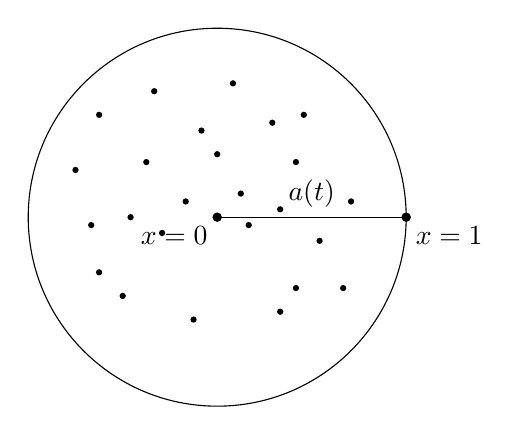
\begin{tikzpicture}[scale=1.0]
\draw (0,0) circle (2.4);
\foreach \x/\y in {-1.5/1.3,-0.8/1.6,0.2/1.7,1.1/1.3,-1.8/0.6,-0.9/0.7,0.0/0.8,1.0/0.7,1.7/0.2,-1.6/-0.1,-0.7/-0.2,0.4/-0.1,1.3/-0.3,-1.2/-1.0,-0.3/-1.3,0.8/-1.2,1.6/-0.9,-0.2/1.1,0.7/1.2,-1.1/0.0,0.8/0.1,-1.5/-0.7,1.0/-0.9,-0.4/0.2,0.3/0.3}
  {\fill (\x,\y) circle (0.04);}
\fill (0,0) circle (0.06);
\fill (2.4,0) circle (0.06);
\draw (0,0)--(2.4,0);
\node[below left] at (0,0) {$x=0$};
\node[below right] at (2.4,0) {$x=1$};
\node[above] at (1.2,0) {$a(t)$};
\end{tikzpicture}
\caption{Clean reconstruction of the homogeneous sphere used in the lecture. The geometry is simple, but it is the whole point: the cosmological scale factor is introduced as the physical distance to the particle at \(x=1\).}
\end{figure}

\section{Energy Conservation and the Friedmann Equation}

Now we write down the energy of that particle. Susskind chooses the mass of the particle to be one, so that we do not have to carry around a test mass which would cancel in the end anyway. The kinetic energy is therefore just
\begin{equation}
\frac{1}{2}\dot a^2.
\end{equation}

The enclosed mass is the volume of the sphere times the density:
\begin{equation}
M_{\mathrm{enc}}=\frac{4\pi}{3}a^3\rho.
\end{equation}
Here \(\rho\) is initially the mass density in the Newtonian discussion. The gravitational potential energy is
\begin{equation}
-\frac{G M_{\mathrm{enc}}}{a}
=
-\frac{4\pi G}{3}a^2\rho.
\end{equation}
The first board frame shows this expression only partially, so we restore the factor of \(G\) and the power of \(a\) from the spoken derivation rather than from the chalk alone.

Thus the total energy takes the form
\begin{equation}
E=\frac{1}{2}\dot a^2-\frac{4\pi G}{3}a^2\rho,
\end{equation}
and Newton tells us that \(E\) is constant in time. Susskind first names that constant in a slightly shifting way, then normalizes it into the standard cosmological notation. If we multiply by \(2\), absorb the constant into a symbol \(k\), and divide through by \(a^2\), we obtain the cleaned Friedmann form
\begin{equation}
\left(\frac{\dot a}{a}\right)^2=\frac{8\pi G}{3}\rho-\frac{k}{a^2}.
\end{equation}
The quantity \(\dot a/a\) is the Hubble parameter \(H\), or as Susskind puts it, the Hubble constant that is not really constant.

\begin{figure}[ht]
\centering

\includegraphics[width=0.56\textwidth]{lecture_03_figure_03.png}
\caption{Boxed curvature term in the Friedmann equation. The screenshot is mainly evidence that the contribution \(-k/a^2\) was explicitly isolated and emphasized on the board.}
\end{figure}

At this point the lecture makes a brief but important pivot toward Einstein. The claim is not that general relativity has been rederived on the spot. The claim is more modest and more useful: for an expanding homogeneous universe, the Friedmann equation is the time-time Einstein equation in disguise. In schematic form,
\begin{equation}
R_{00}-\frac{1}{2}g_{00}R \propto T_{00}.
\end{equation}
The exact coefficients are not derived here, and the board frame does not securely witness them. But the orientation is clear: if we evaluate the left-hand side for an expanding metric, we get the combination involving \(\dot a/a\) and \(k/a^2\), while the right-hand side is the energy density. In Susskind's phrase, we have not abandoned Albert for Isaac; at this stage Isaac and Albert are saying the same thing.

\section{Matter-Dominated Cosmology}

Once the equation is in hand, the next question is immediate: what is \(\rho\)? The lecture first answers that in the matter-dominated case. We take a comoving unit cube, one coordinate unit on a side. Its physical side length is \(a(t)\), so its physical volume is \(a^3(t)\). If the matter simply moves with the cosmic flow, then matter neither enters nor leaves this comoving box, and the total mass inside it stays constant. Let us call that constant \(M\). Then
\begin{equation}
\rho_m=\frac{M}{a^3}.
\end{equation}

This is what Susskind means by a matter-dominated universe: the energy in the box is dominated by particles essentially at rest in the comoving frame. In this idealization the pressure is negligible and one may even think of the temperature as vanishingly small compared with the rest energies involved. He is careful, however, to note that this does not describe the full present-day universe, which is dominated by dark energy; it describes the ordinary matter sector and, historically, a long era in cosmic expansion.

Observationally, \(k\) is very close to zero, so we take \(k\approx 0\) as a good approximation and write
\begin{equation}
\left(\frac{\dot a}{a}\right)^2=\frac{8\pi G}{3}\frac{M}{a^3}.
\end{equation}
The lecture now solves this by the standard honorable method: guess a power law,
\begin{equation}
a(t)=Ct^p.
\end{equation}
Then
\begin{align}
\dot a &= Cp\, t^{p-1},\\
\frac{\dot a}{a} &= \frac{p}{t},\\
\left(\frac{\dot a}{a}\right)^2 &= \frac{p^2}{t^2}.
\end{align}
Substituting into the Friedmann equation gives
\begin{equation}
\frac{p^2}{t^2}=\frac{8\pi G}{3}\frac{M}{C^3 t^{3p}}.
\end{equation}
The two sides can match for all \(t\) only if the powers agree, so
\begin{equation}
3p=2,
\qquad\text{hence}\qquad
p=\frac{2}{3}.
\end{equation}
Therefore the matter-dominated universe expands as
\begin{equation}
a(t)\propto t^{2/3}.
\end{equation}
If we also match coefficients, the bookkeeping constant is
\begin{equation}
C^3=6\pi G M.
\end{equation}

This is one of the central results of the lecture. The scale factor does not grow linearly with time. It grows more slowly, like the two-thirds power.

\section{Radiation-Dominated Cosmology}

Earlier in the universe, the dominant contribution to the energy density was not matter but radiation. Susskind motivates this physically rather than formally. The universe is filled with photons; indeed, in number there are vastly more photons than baryons. Today their energies are tiny, but if we run the universe backward and squeeze the wavelengths, the photons become more and more energetic.

So we take again a comoving unit box. Unlike the matter case, photons move through the box, but on average as many enter as leave, so the average number of photons inside remains roughly constant. The energy of a photon is
\begin{equation}
E_\gamma=h\nu=\frac{hc}{\lambda}.
\end{equation}
The lecture then makes the central dynamical assumption: as the universe expands, the wavelength stretches with it,
\begin{equation}
\lambda\propto a.
\end{equation}
Therefore the energy of each photon scales as
\begin{equation}
E_\gamma\propto a^{-1}.
\end{equation}
Since the average number of photons in the comoving box stays fixed, the total photon energy in the box also scales like \(a^{-1}\). Dividing by the physical volume \(a^3\), we obtain
\begin{equation}
\rho_r\propto a^{-4}.
\end{equation}

This extra power of \(a\) is the whole story. Matter dilutes only because volume grows; radiation dilutes both because volume grows and because each photon's energy redshifts.

Accordingly, the radiation-dominated Friedmann equation is
\begin{equation}
\left(\frac{\dot a}{a}\right)^2=\frac{8\pi G}{3}\frac{M_r}{a^4},
\end{equation}
where \(M_r\) is simply a constant setting the scale of the radiation energy density. The lecture reuses the letter \(m\) here, but it no longer means mass in the earlier sense, so it is cleaner to rename it.

We solve again by the same ansatz \(a(t)=Ct^p\). Then the left-hand side still scales as \(t^{-2}\), while the right-hand side scales as \(t^{-4p}\). Matching exponents gives
\begin{equation}
4p=2,
\qquad\text{so}\qquad
p=\frac{1}{2}.
\end{equation}
Hence the radiation-dominated universe expands as
\begin{equation}
a(t)\propto t^{1/2}.
\end{equation}
If we keep the coefficient, then
\begin{equation}
C^4=\frac{32\pi G}{3}M_r.
\end{equation}

\subsection{Question \& Answer}

\paragraph{Question.} Photons have no rest mass. Why is there still a factor of \(G\) in the radiation equation?

\paragraph{Answer.} Because the source of gravity is not rest mass by itself but energy density. For slow particles, rest mass and energy are essentially the same thing, so Newtonian language is good enough. For photons they are not. A photon has no rest mass, but it certainly has energy, and that energy gravitates. Susskind's preferred image is a box full of radiation: accelerate the box, and it resists more than an empty box. In that sense it has more inertia; and by the equivalence principle, more inertia means more weight. The Einstein equations summarize this by placing energy, momentum, and stress on the right-hand side, not merely rest mass.

\paragraph{Question.} If each photon loses energy as the universe expands, what has happened to conservation of energy?

\paragraph{Answer.} The lecture insists that the Friedmann equation itself is the conservation law. One should not isolate the photon sector and demand that it be constant by itself. In the Newtonian rewriting there is kinetic energy of the expansion and gravitational potential energy as well. The redshifting of the photon bath is part of the full bookkeeping, not a violation of it. In modern language one would say that global energy conservation in an expanding spacetime is subtler than in ordinary mechanics; in the lecture's language, the loss of photon energy is balanced by the energy of the expansion and the gravitational field.

\section{Matter-Radiation Equality and the Change of Expansion Law}

Once both scaling laws are on the board, the lecture turns from algebra to comparison. Matter has
\begin{equation}
\rho_m\propto a^{-3},
\end{equation}
while radiation has
\begin{equation}
\rho_r\propto a^{-4}.
\end{equation}
Therefore radiation dominates when \(a\) is small, and matter dominates when \(a\) is large. This is not a separate theorem added afterward; it is the direct physical meaning of the extra factor of \(a^{-1}\) coming from redshift.

\begin{figure}[ht]
\centering

\includegraphics[width=0.68\textwidth]{lecture_03_figure_05.png}
\caption{Axes for the energy-density plot. The screenshot preserves the board moment at which Susskind begins the graphical comparison of matter and radiation.}
\end{figure}

\begin{figure}[ht]
\centering
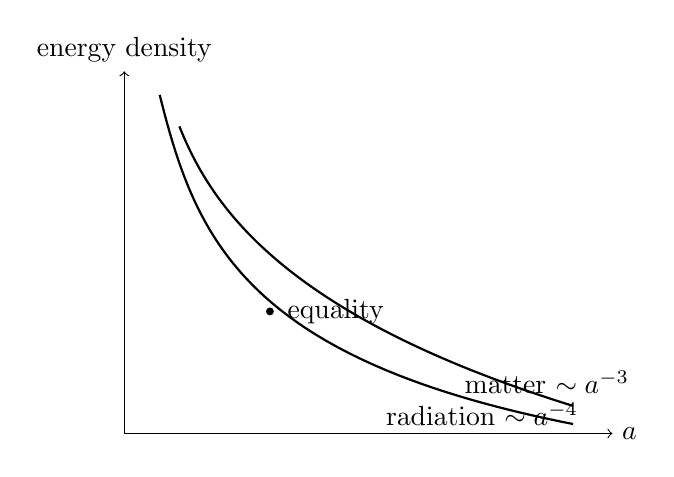
\begin{tikzpicture}[scale=1.0]
\draw[->] (0,0) -- (6.2,0) node[right] {$a$};
\draw[->] (0,0) -- (0,4.6) node[above] {energy density};
\draw[thick] (0.7,3.9) .. controls (1.1,2.9) and (2.0,1.5) .. (5.7,0.35);
\draw[thick] (0.45,4.3) .. controls (0.9,2.5) and (1.5,0.95) .. (5.7,0.12);
\fill (1.85,1.55) circle (0.05);
\node[right] at (1.95,1.55) {equality};
\node[right] at (4.2,0.65) {matter \(\sim a^{-3}\)};
\node[right] at (3.2,0.25) {radiation \(\sim a^{-4}\)};
\end{tikzpicture}
\caption{Transcript-derived reconstruction of the matter and radiation energy densities versus scale factor. The steeper radiation curve dominates at small \(a\), the matter curve at large \(a\).}
\end{figure}

In time language the two asymptotic laws are
\begin{equation}
a(t)\sim t^{1/2}\qquad\text{early},\qquad
a(t)\sim t^{2/3}\qquad\text{later}.
\end{equation}
Susskind gives a lecture-level estimate that the transition from radiation domination to matter domination happened after roughly \(10^4\) years.

\subsection{Question \& Answer}

\paragraph{Question.} Does the exponent \(p\) jump abruptly from \(1/2\) to \(2/3\)?

\paragraph{Answer.} No. The exponents \(1/2\) and \(2/3\) describe two limiting regimes, not two exact laws patched together with a discontinuity. The universe passes continuously through a transition region in which neither pure radiation nor pure matter completely dominates. The effective growth law changes over a relatively narrow interval, but it does not jump. This is exactly why Susskind draws the plots: the comparison is easier to understand geometrically than by trying to force a single exact power law across the whole history.

\section{Temperature, Ionization, and the Surface of Last Scattering}

Before returning to the exact equality time, the lecture pivots to temperature. This is a natural move, because once photon wavelength scales like \(a\), so does the characteristic photon energy. In the lecture's level of approximation, the radiation temperature is proportional to the energy of a typical photon, and therefore
\begin{equation}
T\propto a^{-1}.
\end{equation}

Now we compare two temperatures. Today the cosmic radiation temperature is about \(3\,\mathrm{K}\). The ionizing temperature, taken roughly as the temperature near the surface of the sun, is about \(3000\,\mathrm{K}\). Thus
\begin{equation}
\frac{a_{\mathrm{today}}}{a_{\mathrm{ion}}}\sim 10^3.
\end{equation}
After radiation domination ends, the universe grows approximately as \(a\propto t^{2/3}\), so Susskind estimates the ionization time from
\begin{align}
\left(\frac{t_{\mathrm{today}}}{t_{\mathrm{ion}}}\right)^{2/3} &\sim 10^3,\\
\frac{t_{\mathrm{today}}}{t_{\mathrm{ion}}} &\sim 1000^{3/2}\sim 3\times 10^4.
\end{align}
Taking \(t_{\mathrm{today}}\sim 10^{10}\) years at the order-of-magnitude level, one finds
\begin{equation}
t_{\mathrm{ion}}\sim 3\times 10^5\ \mathrm{years}.
\end{equation}

This is a lecture estimate, not a modern precision number, but it is enough for the physics. Before that epoch the universe was hot enough to ionize hydrogen and helium. It was a plasma: electrons and nuclei moved freely, electromagnetic radiation scattered strongly, and the universe was opaque. After the temperature dropped sufficiently, electrons combined with nuclei to make neutral atoms, the plasma disappeared, and the universe became transparent enough for photons to free-stream over cosmological distances.

That transition region is called the surface of last scattering. The phrase should not mislead us into thinking of a sharp geometric wall. It is really a fuzzy shell in space, or equivalently a fuzzy interval in cosmic time, across which the universe changes from opaque plasma to transparent neutral gas. When we look outward, we are also looking backward in time, so eventually every line of sight reaches that surface. Beyond it, electromagnetic radiation does not give us a clean view.

The lecture then broadens the observational horizon. A neutrino telescope, if one could build an adequate one for such low-energy relic neutrinos, would see earlier than photons, because neutrinos decouple sooner. A graviton telescope would in principle see earlier still. But for electromagnetic astronomy the surface of last scattering is the practical horizon, and what we call the cosmic microwave background is precisely the radiation arriving to us from that shell.

A useful refinement from the question period is that a blackbody's full energy density scales more steeply than its temperature:
\begin{equation}
n_\gamma\propto T^3,
\qquad
\rho_\gamma\propto T^4.
\end{equation}
The first factor counts photons per unit volume; the second combines the number density with the energy per photon.

\subsection{Question \& Answer}

\paragraph{Question.} If the universe was once as hot as the surface of the sun in every direction, why is the night sky not blinding?

\paragraph{Answer.} Because the source we are looking at is not at rest relative to us. The last-scattering surface is receding, and the photons arriving from it have been redshifted by roughly the same factor by which the scale factor has grown since recombination. A \(3000\,\mathrm{K}\) radiation field redshifted by a factor of about \(10^3\) becomes a \(3\,\mathrm{K}\) microwave background. The lecture presents this as a modern form of Olbers' paradox. The resolution is not that the early universe was dim; it was that the photons were stretched on the way to us until they became cold microwaves instead of visible, eye-burning light.

\section{Dark Matter from Galactic Dynamics}

Only after this cosmological spine is in place does the lecture return to the subject promised at the beginning: dark matter. The shift in scale is explicit. Dark matter was not first inferred from cosmology in the large-scale sense, but from astronomy, by looking at galaxies and measuring what are called their rotation curves.

We begin with the simplest Newtonian problem. Suppose a light object orbits a central mass \(M\) at radius \(r\). The gravitational force is
\begin{equation}
\frac{GMm}{r^2},
\end{equation}
and the centripetal acceleration for circular motion is \(v^2/r\). Equating force to mass times acceleration, we find
\begin{equation}
\frac{v^2}{r}=\frac{GM}{r^2},
\end{equation}
so
\begin{equation}
v(r)=\sqrt{\frac{GM}{r}}.
\end{equation}
Thus if most of the mass is concentrated near the center, the orbital speed should fall like \(r^{-1/2}\). That is the familiar Keplerian behavior of the solar system.

\begin{figure}[ht]
\centering
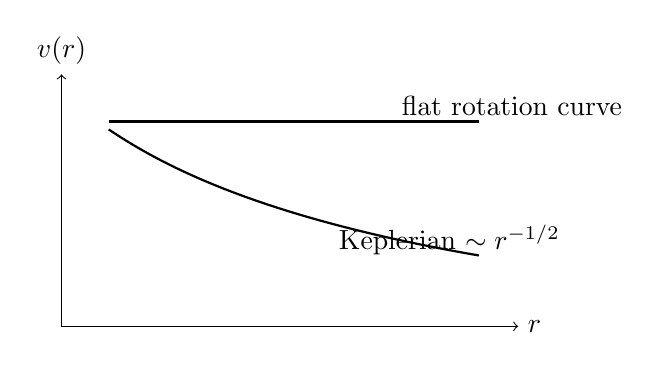
\begin{tikzpicture}[scale=1.0]
\draw[->] (0,0) -- (5.8,0) node[right] {$r$};
\draw[->] (0,0) -- (0,3.2) node[above] {$v(r)$};
\draw[thick] (0.6,2.6) -- (5.3,2.6);
\draw[thick] (0.6,2.5) .. controls (1.2,2.1) and (2.4,1.4) .. (5.3,0.9);
\node[right] at (4.2,2.8) {flat rotation curve};
\node[right] at (3.4,1.1) {Keplerian \(\sim r^{-1/2}\)};
\end{tikzpicture}
\caption{Transcript-derived comparison between the Keplerian falloff expected from centrally concentrated mass and the approximately flat rotation curves observed in large galaxies.}
\end{figure}

But galaxies do not behave this way. If one assumes that mass follows light, so that most of the mass sits where most of the visible matter sits near the galactic core, then the outer stars should slow down. Instead the measured orbital speeds are roughly constant over a large range of radii.

The natural repair is to replace the central mass \(M\) by the enclosed mass \(M(r)\):
\begin{equation}
\frac{v^2}{r}=\frac{G M(r)}{r^2}.
\end{equation}
If \(v(r)\) is approximately constant, then this implies
\begin{equation}
M(r)\propto r.
\end{equation}
That is already strong evidence that the visible light is not tracing all the gravitating matter.

Assuming a roughly spherical halo, the enclosed mass is related to the density profile by
\begin{equation}
M(R)=\int_0^R 4\pi r^2 \rho(r)\,dr.
\end{equation}
If \(M(R)\propto R\), then differentiating with respect to \(R\) gives
\begin{equation}
4\pi R^2 \rho(R) \propto 1,
\end{equation}
and therefore
\begin{equation}
\rho(r)\propto \frac{1}{r^2}.
\end{equation}
So the lecture arrives at a simple picture: a galaxy is embedded in a large, approximately spherical dark halo whose density falls gradually rather than collapsing sharply with the luminous disk. The total mass inferred in this way is only heuristic at lecture level, but the point is robust: a galaxy is several to ten times heavier than what one would estimate from luminous matter alone.

At this stage the lecture makes a second, more qualitative inference. Whatever this matter is, it does not shine, and it does not dissipate efficiently. Ordinary baryonic matter cools, collides, radiates, and collapses into denser structures. Dark matter evidently does not do that in the same way. It stays in a large halo.

\subsection{Question \& Answer}

\paragraph{Question.} If the dark halo is so massive, why does it not dissipate and collapse together with the luminous matter?

\paragraph{Answer.} Because collapse requires dissipation. A gas cloud shrinks not merely because gravity pulls inward, but because collisions and radiation allow energy to be shed. Ordinary matter has many ways to do this: atoms collide, charges radiate, energy escapes, and the cloud can settle into a disk or a star. Dark matter appears to be almost collisionless and almost non-radiating. It has kinetic energy, but no efficient mechanism for bleeding that energy away. In the lecture's analogy, the Earth does not fall directly into the sun because there is essentially no friction. Dark matter likewise remains in extended orbits, not necessarily circular ones, precisely because it does so little besides gravitate.

The lecture is careful not to oversell the detailed halo dynamics. Susskind explicitly says that he does not know a simple first-principles derivation of the \(1/r^2\) profile, nor does he claim detailed knowledge of halo rotation or structure. That boundary should be preserved. What is sharp is the inference from flat rotation curves to extra gravitating matter; what is not yet sharp, in this lecture, is the full dynamical theory of halo formation.

The section closes with a more decisive observational argument: the Bullet Cluster. In a collision of galaxy clusters, the hot ordinary gas interacts strongly and is seen separately, while the dominant gravitating mass inferred by lensing passes through more nearly collisionlessly. Thus the mass distribution becomes spatially separated from the luminous baryonic matter. This is precisely what one would not expect if the whole effect were only a modification of Newton's law attached to visible matter. The Bullet Cluster does not tell us what dark matter is, but it argues strongly that there really is unseen gravitating matter.

\section{Summary}

The lecture begins with one simple equation and then repeatedly changes the physical meaning of its source term. In a homogeneous universe, Newtonian energy conservation leads to the Friedmann equation; in Einstein's language the same equation is the time-time field equation. Matter at rest in a comoving box gives \(\rho_m\propto a^{-3}\) and \(a(t)\propto t^{2/3}\). Radiation, because each photon's wavelength stretches with the universe, gives \(\rho_r\propto a^{-4}\) and \(a(t)\propto t^{1/2}\). From that follow matter-radiation equality, the cooling law \(T\propto a^{-1}\), the epoch of recombination, and the surface of last scattering.

Only then does the lecture move to galaxies, where Newtonian reasoning reappears in another form. Flat rotation curves imply \(M(r)\propto r\), hence a large dark halo with density roughly \(\rho(r)\propto r^{-2}\). The detailed nature of that halo is left open, but the qualitative picture is not: most of the gravitating matter in and around galaxies is dark, weakly interacting, and very likely particulate rather than a mere modification of the force law.